%\documentclass[letterpaper, 12 pt, conference]{ieeeconf}  % Comment this line out
                                                          % if you need a4paper
\documentclass[a4paper, 10pt, conference]{ieeeconf}      % Use this line for a4
                                                          % paper

\IEEEoverridecommandlockouts                              % This command is only
                                                          % needed if you want to
                                                          % use the \thanks command
\overrideIEEEmargins
% See the \addtolength command later in the file to balance the column lengths
% on the last page of the document

% This is needed to prevent the style file preventing citations from linking to 
% the bibliography
\makeatletter
\let\NAT@parse\undefined
\makeatother

\usepackage[dvipsnames]{xcolor}
\usepackage{footmisc}
\newcommand*\linkcolours{ForestGreen}
\usepackage[dvipsnames]{xcolor}
\usepackage{scrextend}
\usepackage{times}
\usepackage{textcomp}
\usepackage{graphicx}
\usepackage{geometry}
\usepackage{amssymb}
\usepackage{gensymb}
\usepackage{amsmath}
\usepackage{breakurl}
\def\UrlBreaks{\do\/\do-}
\usepackage[breaklinks,pagebackref,colorlinks=false,
linkcolor=black,
filecolor=orange,      
urlcolor=brown]{url,hyperref}
%\usepackage{url,hyperref}
\hypersetup{
colorlinks,
linkcolor=\linkcolours,
citecolor=\linkcolours,
filecolor=\linkcolours,
urlcolor=\linkcolours}

%\usepackage{algorithm}
\usepackage{algorithmic}
\usepackage[linesnumbered,ruled,vlined]{algorithm2e}
\usepackage{algcompatible,lipsum}
\usepackage{caption}
\usepackage[labelfont={bf},font=small]{caption}
\usepackage[none]{hyphenat}

\usepackage{mathtools, cuted}

\usepackage[noadjust, nobreak]{cite}
\def\citepunct{,\,} % Style file defaults to listing references separately

\usepackage{tabularx}
\usepackage{amsmath}

\usepackage{float}

\usepackage{pifont}% http://ctan.org/pkg/pifont
\newcommand{\cmark}{\ding{51}}%
\newcommand{\xmark}{\ding{55}}%

\newcommand*\diff{\mathop{}\!\mathrm{d}}
\newcommand*\Diff[1]{\mathop{}\!\mathrm{d^#1}}
\newcommand*\imgres{600}


\newcolumntype{Y}{>{\centering\arraybackslash}X}

%\usepackage{parskip}

\usepackage[]{placeins}

% \usepackage{epstopdf}
% \epstopdfDeclareGraphicsRule{.tif}{png}{.png}{convert #1 \OutputFile}
% \AppendGraphicsExtensions{.tif}

\newcommand\extraspace{3pt}

\usepackage{placeins}

\usepackage{tikz}
\newcommand*\circled[1]{\tikz[baseline=(char.base)]{
            \node[shape=circle,draw,inner sep=0.8pt] (char) {#1};}}
            
\usepackage[framemethod=tikz]{mdframed}

\usepackage{afterpage}
\usepackage{stfloats}

\usepackage{atbegshi}
\newcommand{\handlethispage}{}
\newcommand{\discardpagesfromhere}{\let\handlethispage\AtBeginShipoutDiscard}
\newcommand{\keeppagesfromhere}{\let\handlethispage\relax}
\AtBeginShipout{\handlethispage}
\usepackage[export]{adjustbox} % loads also graphicx
\usepackage{comment}

\title{ \bf SASSCAL WebSAPI: A Web Scraping Application Programming Interface to Enhance The SASSCAL Weathernet
}

\author{Tsaone Swaabow Thapelo$^{*1}$,  Molaletsa Namoshe$^{2}$,  Oduetse Matsebe$^3$,\\
Tshiamo Motshegwa$^4$, Mary-Jane Morongwa Bopape$^5$  \\
%Department of Mechanical, Energy and Industrial Engineering$^{1,3,5}$\\
	%Department of Mechanical, Energy, and Industrial Engineering $^{1,2,3}$\\
	Botswana International University of Science and Technology$^{1,2,3}$\\
	%	Department of Computer Science, 
		University of Botswana$^4$\\
			South African Weather Services, Pretoria, South Africa $^{5}$ \\
		{*\color{black}Corresponding Author}: {\color{black}swaabow@gmail.com}
}



\setlength{\columnsep}{1cm}
\newgeometry{layoutwidth  = 8.2500in,
	layoutheight = 11.20in,
	vmargin      = 00.50in, %Inches at top
	hmargin      = 00.60in,
	headheight   = 00.50in,
	headsep      = 00.15in,
	footskip     = 00.60in}
\pdfpagewidth  = 8.2500in
\pdfpageheight = 12.00in

\begin{document}

\maketitle
\thispagestyle{empty}
\pagestyle{empty}


%%%%%%%%%%%%%%%%%%%%%%%%%%%%%%%%%%%%%%%%%%%%%%%%%%%%%%%%%%%%%%%%%%%%%%%%%%%%%%%%
\begin{abstract}
\noindent
The Southern African Science Service Centre for Climate and Land Management (SASSCAL)  was initiated to support regional weather monitoring and climate research  in southern Africa.
As a result, several Automatic Weather Stations (AWSs) were implemented to provide numerical weather data within the collaborating countries. 
%Problem
 Meanwhile, access to the SASSCAL weather data is limited to a number of records that are achieved via a series of clicks. 
 Currently, end users can  not efficaciously extract the desired weather values. 
Thus, the data is not fully utilised by end users. % like students, researchers, contractors and local meteorologists. 
 % one sentence about research/study objective,
 This work  contributes with an open source Web Scraping Application Programming Interface (WebSAPI) through an interactive dashboard. 
 The objective is to extend functionalities of the SASSCAL weathernet for: data extraction, statistical data analysis and visualisation. %generating data sets that is ingestible to data mining workbenches for further statistical analyses. 
 %Methods
  The SASSCAL WebSAPI    was developed using the R statistical environment. 
  It deploys  web scraping and data wrangling techniques to enhance access to SASSCAL weather data and  ultimately generate desired data sets.  
 %Results
% The generated tables and figures can be exported as .csv or .pdf files. %A hypothetical dataset was used to demonstrate the application of the SASSCAL WebSAPI.
 %conclusion
 This WebSAPI reduces the risk of human error, and the researcher's effort of generating data sets.  %The overall gain is the  efficacious use of the data collected by the  AWSs maintained through the SASSCAL initiative. 
  % a sentence about the significance of that finding.
  The WebSAPI is   useful for meteorologists, environmental researchers; or in any other research projects that require   the SASSCAL weather data.  %
\\
\\
\emph{Key Words}:  SASSCAL,  WebSAPI, Web Scraping, Dashboard
\end{abstract}

%%%%%%%%%%%%%%%%%%%%%%%%%%%%%%%%%%%%%%%%%%%%%%%%%%%%%%%%%%%%%%%%%%%%%%%%%%%%%%%%
\section{Introduction}
\label{Intro}
\noindent
Automatic Weather Stations (AWSs) provide numerical weather data that has potential to catalyse the development of robust responses to   climate related problems. For that main reason, the Southern African Science Service Centre for Climate and Land Management (SASSCAL)\footnote{\url{http://www.sasscalweathernet.org}\label{weathernet}}  was initiated to support regional weather monitoring and climate research in southern Africa. The SASSCAL weathernet (see Fig \ref{SASSCA}) disseminates near to real time weather data (i.e., since 2014 in Botswana) from AWSs at various temporal resolutions (quarterly, hourly, daily and monthly).   The collected data include, but not limited to: temperatures, solar radiation, relative humidity and sunshine duration. Such weather data is vital in environmental data science \cite{GIBERT20183}. % and other applied works (i.e., smart energy management systems \cite{aguera2018weather}).  
\\
   	\\
   	   The SASSCAL weather data can be integrated with data from different sources for research purposes. For instance, Moses \textit{et. al.} \cite{moses2018effects}   merged the SASSCAL data with other  meteorological data from the Botswana Department of Meteorological Services  to analyse  effects of  solar radiation, wind speed and  humidity 	on evapo-transpiration around the Okavango Delta.  Similarly, daily maximum temperature values are vital in the understanding of heatwaves \cite{moses2017heat}; while rainfall values %from the SASSCAL weathernet 
   	   can help in  assessing rainfall erosivity \cite{singh2020assessing}. % at locations of interest covered by the AWSs.
   	   \newpage
\begin{figure}[tbh!]
\centering
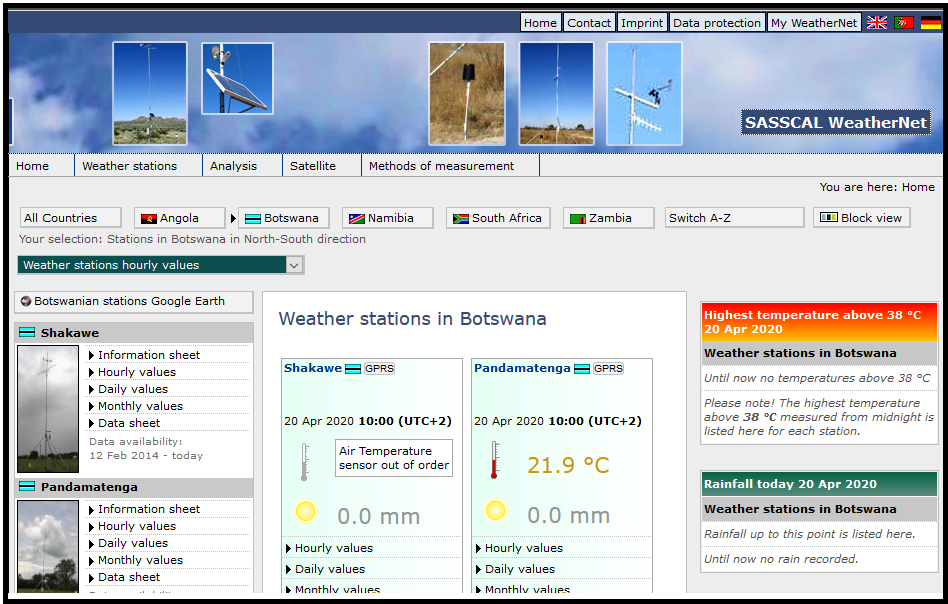
\includegraphics[width=1\columnwidth]{fig/Sasscalweathernet.png}
\caption{Visualisation of  AWS data via the SASSCAL weathernet.}
\label{SASSCA}
\end{figure}
\noindent
	The SASSCAL weathernet  in \ref{weathernet} disseminates  observed weather variables from various AWSs across the five collaborating countries (Angola, Botswana, Namibia, South Africa and Zambia). 
%	Likewise, a researcher may wish to follow previous works \cite{singh2020assessing} and use rainfall values from the SASSCAL weathernet to assess rainfall erosivity at locations of interest covered by the AWSs. %However, the SASSCAL weathernet is still new, with limited historical data for meaningful climate studies.
	%Meanwhile, it has the potential to catalyse   many research projects in the world of work. 
	Despite the distinct potential use of the SASSCAL weather data, there is a burden on the end users to access, download and use such data in research (see Fig. \ref{datamunging}). % Currently, users can only
	%The current access mechanisms deployed by the SASSCAL weathernet \ref{weathernet} only allow end users to
%Currently, end users can 	view weather data and manually download  subsets of data at a time following steps in Fig. \ref{datamunging}. % using a set of clicks. % (see Fig. \ref{datamunging}).
	First, the user has to navigate to the SASSCAL weathernet to identify a country of interest, the    AWS name of interest; and the temporal resolution of the SASSCAL weather data. % (hourly, daily or monthly).
The user can then manually copy and paste the whole data to a storage file for data analysis. There is an option to download the SASSCAL weather data in excel format only. %(currently not working). % as seen in Fig. \ref{BugUno}).
	%Even when this option is working, the steps of downloading the data are not obvious to new users. 
	However, there is no option to only select the desired weather values. 
	%All these challenges  	limit the 	effective 	use of these weather data in specific  projects.
	\begin{figure}[h]
   		\centering
   		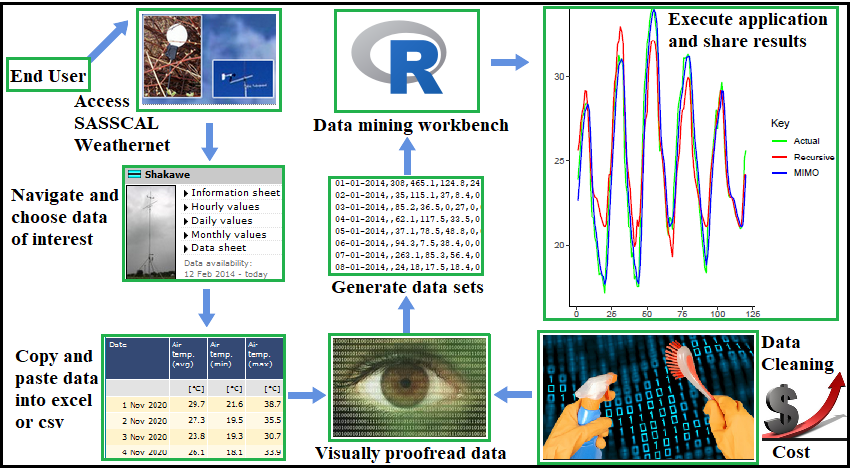
\includegraphics[width=0.98\linewidth]{fig/MiPipe}
   		\caption{Manually extracting data  from the  SASSCAL weathernet}
   		\label{datamunging}
   	\end{figure}
   	
\noindent  
   	 This repetitive manual collection of data is costly, time consuming and error-prone. % The situation worsens when extracting finer grained temporal data   from multiple AWSs.   
   	 Even after downloading the weather data, end users face a challenge of generating clean data sets containing the desired variables for further use. % in their projects. %  All these invite techniques of data science. %web scraping, data wrangling and dashboard applications 
   	 %to extend the functionalities of the SASSCAL weathernet. % to serve  users.
  % 	 \newpage
   %	 \noindent
  % 	 %	However, extraction of  the desired SASSCAL weather  data by end users  is not efficacious as discussed in section \ref{Intro}. 
%	
%		\begin{figure}[h]
  % 		\centering
  % 		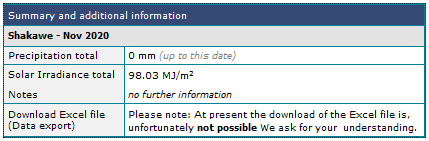
\includegraphics[width=1\linewidth]{fig/BugUno}
  % 		\caption{The SASSCAL download option currently not working}
  %% 		\label{BugUno}
 %  	\end{figure}
%	
%	\noindent
%	Currently, there are no web scrapers in existence to enhance efficacious access to the SASSCAL  weather data. 
	%To address this gap, this work deploys the basic concepts of web scraping in \cite{yang2010development,glez2014web,BONIFACIO201513,bradley2019web} to develop the SASSCAL WebSAPI  for  visualisation and downloading of  consecutive SASSCAL  weather data of interest. 
	% These limit the use of the SASSCAL data in research. \\
%	 \\
   	 This work presents the SASSCAL Web Scraping Application Programming Interface (WebSAPI). The main objective is to enable end users to: (1) access and visualise weather data from the   SASSCAL weathernet; and (2) download desired data sets for further use in other data driven projects. Web scraping \cite{WebSrapping} is a data science technique that deploys scripts for extraction and consolidation of structured data from websites to meet end users' requests. A script is a computer program that automates a specific task following some selected programming languages like R or Python. Thus, a WebSAPI can be seen as an application service that allows access to online data for further use in research projects.
\\
\\
The structure of the work is as follows. Section \ref{LR} presents related literature, while section \ref{Metodologia} presents the   approach deployed in the development of the SASSCAL WebSAPI. % and its basic functionalities. 
   Section \ref{Resul} presents results. It also illustrates how the SASSCAL WebSAPI can be used to enhance the extraction of weather variables and ultimately analyse temperature patterns at the Shakawe weather station. %around the Okavango Delta. %as an example of the benefits of having enhanced tools for web scrapping tools. 
Section \ref{Discus} discusses the outputs of this work, including some  limitations. Section \ref{Conclu} concludes the work, with  recommendations and future directions presented in sections \ref{Reco} and \ref{Futuro} respectively.
%including the implications and limitations of the SASSCAL WebSAPI. 
   %Section \ref{Conclu} presents   conclusions and future from this work. % resulting from this work.
   
\section{Related Literature Review}
\label{LR}
\noindent
 	Web scraping techniques have been widely deployed in a number of projects from different disciplines such as in health economics \cite{smith2020making} and climate science \cite{yang2010development}. Regardless of the discipline, the general idea is to allow greater visibility, access, extraction and usability of the online data.  This work is similar to the work in \cite{BONIFACIO201513}, who presented a free tool for automated extraction and consolidation of climate data from different online web data banks.   A similar work by Yang \emph{et. al.} \cite{yang2010development} presented a system with functionalities for scraping, filtering and visualising climatic data for easy use.   This work is related to \cite{sitterson2020demonstration} regarding the user API for data request.
 	It is also similar to \cite{BONIFACIO201513} in such it deconstructs the URL for a given station and then modifies the date range and the desired temporal resolution to extract desired data. 
\\
\\
It should be noted that   most of these works discussed so far are case specific; and  each business problem has different objectives based on specific data sources with different data types. 
 	Therefore each problem requires targeted solutions using specific platforms and software for data management, data visualisation, data analysis and dissemination of outputs. To that point, the work in \cite{li2020towards} argues that modern environmental decision support systems implementation should be more flexible, user-friendly and simple to deploy. 
 Unlike the mentioned works,  work this deploys the state of art programming language (R) that is simple to deploy.
 A number of previous work deploying the R statistical computing environment were discussed in \cite{li2020towards}. \\
 	\\
     This work contributes by addressing the second ``pillar" of the Global Framework for Climate Services \cite{VAUGHAN201665} using climate informatics. Climate informatics \cite{lyubchich2019statistics,GIBERT20183}
 is new discipline that requires    collaborations between mechatronics engineers, climate scientists, data scientists,
statistical machine learning researchers, and developers in order to bridge this gap between data and
the targeted end users.
% to enhance the generation, delivery, and making use of climate data, according to end  user needs and agreed standards \cite{VAUGHAN201665}. 
     
%\\
  %   \\
%     This paper describes the SASSCAL WebSAPI, its components as well as its underlying design principles. The initial idea started in 2014 when the SASSCAL weathernet was less than six months old. By then, the collected data was not enough for meaningful data science and predictive analytics projects. This is an ongoing project with a lot of content to articulate in a brief paper. Much focus is on the logic of the API, illustrating how the respective components fit together, with links to more detailed resources.  % for further reading.\\
  
  \newpage
\section{Methodology: Data, Tools and Methods}
	\label{Metodologia}
	\noindent
	The SASSCAL weathernet \ref{SASSCA} provides open weather  data   from Angola, Botswana, Namibia, South Africa and Zimbabwe. The  data is  reviewed for quality control   before dissemination  \cite{kaspar2015sasscal}. % in research and decision making purposes. 
Fortunately, access to the   SASSCAL weather data  is defined using the same abstract pattern.
	Each country (with a unique code) has various AWSs; and each AWS has a unique station identifier (ID). 
	The  home page  $URL$ for each SASSCAL AWS data is	defined by $x/y?z$; where
%	\begin{equation}
%		L = x/y?z.
%		\label{pattern}
%	\end{equation}	
%
%In Eq. \ref{pattern}, % $L$ is the complete $URL$ for the data of interest, 
$x$ is the SASSCAL Weathernet link in \ref{weathernet};
$y$ is just the $weatherstat\_\alpha\_AO\_we.php$ token that defines the weather statistics for a given  resolution  (i.e, hourly, daily or monthly as defined by $\alpha$); and $z$ is the logger ID ($loggerid\_crit=n$), where $n$ is the AWS' unique  ID.  
	The proposed web scraping toolkit is equally useful for end users from all these collaborating countries. However, for demonstration purposes this work only focuses on  the  weather data from Botswana. %, particularly the Shakawe AWS in the Okavango Delta. 
%	\subsection{Data Sources}
	\noindent
	%\subsubsection{Data Sources}

	%especially for non data science end users.
	\subsection{Study Area}
\noindent
Botswana is situated between longitudes 20\textdegree E and 29\textdegree E, and between latitudes 17\textdegree S and 27\textdegree S. %; with a surface area of $\approx$582000$km^2$. 
The country has a hot and semi-arid to arid climate. The highest maximum air temperatures are observed between October and March  (summer period) \cite{moses2017heat,ARCHER201722} with mean monthly  temperatures ranging between 30.9\textcelsius\ and 33\textcelsius. These are normally accompanied by heat waves, with maximum temperatures going up to $\approx$42\textcelsius\ \cite{moses2017heat}. 
Botswana is still under researched regarding weather and climate services. Previous studies \cite{kolawole2014ethno} indicate that the Okavango Delta is experiencing progressive increase regarding temperatures which ultimately lead to increase in potential evapo-transpiration \cite{moses2018effects}.   For that reason, the Okavango Delta located in the north-west was selected as the study area. The weather data was collected from the   Shakawe AWS (WMO No.: 68026, Station ID: 68026). % and Tubu (WMO No.: 68027, Station ID: 67591).

\begin{figure}[h]
	\centering
	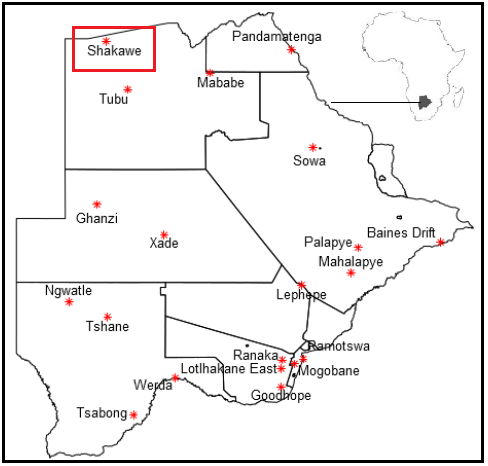
\includegraphics[width=1\columnwidth]{fig/Map20.png}
	\caption{Data source area (Sakawe) in the North-West of Botswana.}
	\label{Shakawe}
\end{figure}

\subsection{Data}
	\noindent
	%\subsubsection{Data Sources}
%The collected data include: air temperature, soil temperature, soil humidity, precipitation,   wind speed, wind direction,   relative humidity, barometric pressure, solar radiation, dew point and leaf wetness. 	
The data set used for demonstrations contains daily (maximum, minimum, and mean) temperature series from the Shakawe AWS, ranging from 01-01-2015 to 31-12-2015.
%\\
%\\

\subsection{Tools and Methods}
\noindent
 This work follows  the data science approach in \cite{wickham2016r,bradley2019web}  %to tailor the CRISP  as seen in  Fig. \ref{Flw}
 using open-source platforms (R\footnote{\url{https://www.r-project.org/}} and RStudio\footnote{\url{https://rstudio.com/}}). % to facilitate reproducibility of results.  R, like Python, is a state of art programming language for data science. 
 R is simple to learn, with a vast number of packages supported by a large community of statisticians and developers. R was chosen because it is the defacto data mining workbench for statistical computing. R has excellent packages for web scraping, data wrangling, data visualisation, and dashboard designs. % of targeted services to end users using scalable dashboard applications. 	
%The following sections articulate in details the main components of the proposed SASSCAL WebSAPI.
%Our SASSCAL WebSAPI toolkit aims to (1)  Find the desired pages containing the requested data by end user; (2) Generate all the subpages that make up the reviews; (3)  Scrape the weather data from each of them; (4)
%The first aim is to  facilitate efficacious extraction of the weather data from the SASSCAL Weathernet. The  SASSCAL  Weathernet was investigated to explore its logical structure. 
%However,  not all of those tables contain the data of interest.   The SASSCAL WebSAPI was developed to  enable the extraction of numerical  values from the desired HTML tables on the SASSCAL Weathernet. 
% \newpage
The main components of this toolkit comprise: a (1) Data Requester: enables the processing of the SASSCAL Weathernet link to  determine the pages containing the requested weather data; (2) Data Fetcher: to extract the SASSCAL weather data from the selected pages.; (3) Data Parser: to deconstruct and parse the contents of the \emph{HTML} file; (4) Data Wrangler: to combine the weather data into a  data frame; (5)  Dataset Generator: to generate  data sets; and  (6) the Communicator: implements  a dashboard  to disseminate the weather outputs to end users (see Fig. \ref{Flw}).  
%The Data Fetcher  % based on the request from the Data Requester. 
%The Data Parser  
%The Data Wrangler  
%The  Communicator  %to visualise,  explore and download weather data. %the  weather data. %It serves as an interface between the end user and the data availed by the SASSCAL Weathernet. 

\begin{figure}[h]
		\centering
		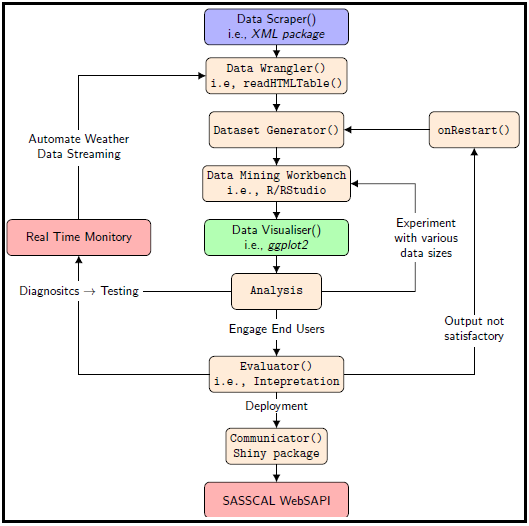
\includegraphics[width=1\linewidth]{fig/MiPipeLine}
		\caption{Workflow of the  SASSCAL WebSAPI}
		\label{Flw}
	\end{figure}
\noindent

\subsection{Web Scraping, Data Preparation and Data Visualisation}
\noindent
The  \emph{XML} package \cite{lang2013package}  was used  to parse a given \emph{URL} and create a Document Object Model ($html\_DOM$)  as seen in Algorithm \ref{WebScraper}.
%Unlike the RCurl and Rvest, t
The % advantage of using the 
XML package  deploys the $readHTMLTable()$ function which can be used to  specify weather observations to  select from  the HTML tables in the SASSCAL weathernet. 
% The $html\_DOM$ enables the: (1) creation  of derived documents, (2) navigation within the HTML  structure, (2) manipulation (addition, deletion, modification) of the  elements and content of the HTML web page.
 %This also enables modification of  data types (i.e, date and numeric values) of the  variables.
%\\
%\\
 We used R's $length()$ function to determine the number of tables for a given $html\_DOM$. There are three $html\_DOM$ objects for each temporal resolution ($\alpha$); each with  multiple tables. 
%Some tables contain non-numeric data and information like figures (see Fig. \ref{BugUno}).
%We  extract   tables with numerical values.
%A visual inspection of the SASSCAL Weathernet page reveals that there are several tables used to visualise data and  information. 
There are 14 tables in the $html\_DOM$ corresponding to the web page with the hourly data, and we are interested in the $13^{th}$ table. The $html\_DOM$ corresponding to the web page with the daily observations has   13 tables, with daily values contained in the $12^{th}$ table. The last $html\_DOM$  has 18 tables with  the  monthly numerical weather data of interest  in the $10^{th}$ table.
% using the R and RStudio statistical environment. to extract data from HTM
%  The \emph{tidyverse} is a set of R packages, articulated in \cite{wickham2019welcome}, with common low-level grammar, data structures and API design for data science. 
  %Data science is a generic field that enables users to turn raw   data into useful insight for better understanding and generation of vital knowledge \cite{wickham2016r}. 
%   We deploy the embedded packages in \emph{tidyverse} to allow end users to import  data from the weathernet using the \emph{Data Scraper()} function. % into a data mining workbench as a data frame. 
%Once loaded, the data is transformed (manipulated) using the \emph{Data Wrangler()} function. 
%Table \ref{Tools} shows the   R packages used by the SASSCAL WebSAPI. The \textit{rvest} package \cite{wickham2016package} enables access to the SASSCAL weather data. %  in  this work.
\newpage
\noindent
Algorithm \ref{WebScraper} takes in a  $URL$ to a given AWS with a specified temporal resolution ($\alpha$) as discussed previously.
 %The output is  for  generation of   weather data sets.  
Line 3 facilitates the choice of  desired tables  using the parameter $\beta$ ($beta$ can be 13, 12 or 10 as discussed above). 
We implement the $DataWrangler()$ function to iterate through the table containing  dates of  observations. It uses the $\rho$ argument to determine the date range (i.e., 2015-01-01 to 2019-12-31) for the data of interest. The extracted weather data is then unified into a single data frame to generate   data sets for further use. % for dissemination. % or further applications. % or injection into  a data mining environment. %of interest.

	\begin{algorithm}
		\caption{Web scraping and data wrangling}
		\label{WebScraper}
		\KwIn{URL: of  type \emph{String}}
		\KwOut{A dataset  of numerical weather data}
		\While{(URL is $Valid$)}
		{%miCamino = ``FilePath"\;
			$html\_DOM$ $\leftarrow$ $readHTMLTable(URL)$\\
			%\tcc{Select the desired table}
			$Dataframe$ $\leftarrow$ $as.data.frame(html\_DOM[\beta])$; \\
			$Dataset$ $\leftarrow$ $DataWrangler(Dataframe,\rho)$\\
			% $\leftarrow$ select the desired weather variables;\\
		%	Generated\_Set $\leftarrow$ Create new variables; \\
		%	Dataset $\leftarrow$ append all outputs into a csv file; \\
			
			\KwRet{Dataset}\tcp*{Return the dataset}
		}
	\end{algorithm}
	\noindent

%  	\caption{The core and non-core packages used in this work.}
%  	\centering 
%  	\begin{tabular}{ | >{\raggedright}m{1.5cm} || m{6cm} |} % | m{1.3cm} | }      % centered columns (3 columns) 
%  		\toprule                                   %inserts double horizontal lines 
%  		\textbf{Package} & \textbf{Purpose} \\ % & \textbf{Description} \\  % inserts table heading 
%  		\hline
%  		%\emph{rvest} & for web scraping   \\ \hline
%  		\emph{XML} \cite{lang2013package} & for web scraping and XML parsing \\ \hline
%  		\emph{ggplot2}	& for data visualisation  \\ \hline
%  		\emph{dplyr}	& for data manipulation / transformation  \\ \hline
%  		\emph{readr}	& for data import   \\ \hline
%  		\emph{lubridate}	& for date/times   \\ \hline
%  		\emph{feather}	& for sharing with Python and other languages   \\ \hline
%  		\emph{haven} 	& for SPSS, SAS and Stata files   \\ \hline
%  		\emph{tidyr} & for data tidying  \\ \hline
%  		\emph{readxl} & for operations with .xls and .xlsx files \\ \hline
%  		\emph{magrittr} & for structuring sequences of data operations \\ \hline
%  		\emph{tibble} & for data wrangling  \\ \hline
%  		\emph{stringr} & String manipulation \\ \hline
%  		\emph{rebus} & Verbose regular expressions \\ \hline
%  		\bottomrule
%  	\end{tabular}
%  	\label{Tools}
%  \end{table}



%\newpage
%\noindent
 % extraction of the  SASSCAL weather data and the generation of   datasets.
%The  $read\_html()$ function    takes in as input the $URL$ of the targeted AWS to create a Document Object Model that will hold all the weather data and structure of the targeted SASSCAL web.  We then use the use the $html_nodes()$ function to extract tables of interest.  
%The \emph{Data Wrangler()} method  uses the \emph{dplyr} package \cite{wickham2015dplyr} to provide end users with the functionality of selecting the desired weather variables based on their names.  % The \emph{Dataset Generator()} function  generates consistent formats    for  analysis and modelling. % in goal of these tools is to enable web scraping, data wrangling,  and visualisation. 
 
\subsection{Dashboard Design: The Graphical User Interface (GUI)} 
\noindent
%The SASSCAL weathernet portal in \ref{weathernet} provides a Graphical User Interface (GUI) for dissemination of the climatic data to end users.  As mentioned in section \ref{Intro}, efficacious access to such data is not trivial since end users are required to use a series of clicks and can only download the desired  data using a number of clicks. %The following algorithm completes the download
Algorithm \ref{WebScraper} implements the Data \emp{Requester()} and the  Communicator components.  We implement three functions for the dashboard page:   the $dashboardHeader()$ to define the title (i.e., SASSCAL WebSAPI) and   the $dashboardSidebar()$ to define the two functionalities of  visualising:  the AWS by country, and   the tables of numerical weather data. The $dashboardBody()$  facilitates selection of the AWS, the  resolution, date range, use of data, type of format for exportation, and  desired weather values.  % data and downloading the desired data.
The GUI also visualises data distributions using  violin/Box-plots  \cite{hintze1998violin}.

\begin{algorithm}
	\caption{Dashboard design for dissemination}
	\label{WebScraper}
	\KwIn{It requires Algorithm \ref{WebScraper}.}
	\KwResult{SASSCAL WebSAPI GUI}
	\While{(Interactive)}
	{
		gui $\leftarrow$ fluidPage(
			{%path $\leftarrow$  ``$FP$" %\tr{Assign the file path of the data source}
	%	Table $\leftarrow$  parseTheTables(path) %\tr{Read the data source}
	%
		$F$ $\leftarrow$ DataScraper()   %\tr{Create a dataset $miFichero$ for modelling}
	}\\
		$T$\leftarrow$ dashboardHeader(...),\\
		$SDB$\leftarrow$ dashboardSidebar(...),\\
		$B$$\leftarrow$dashboardBody( fluidRow(...))
		)\;\\
		server $\leftarrow$ function(I,O) \{ Communicator($F$) %	X = Actual$\leftarrow$ tail(MAXTMP[(n-(LB)):n],h)\\
		%	$Model_{KNN} \leftarrow \hat{y} =  \frac{1}{k}\sum_{x_{i=1} \in \aleph_k(x^*)}^{k}x_i,$\\
       %			myPlots $\leftarrow$  PlotFunction(Preds,LosFunc,...)
		\};\\
	%	\vspace{0.1in}
		shinyApp(gui, server)\;
}
\end{algorithm}


\noindent
The raster package \cite{hijmans2015package} and the maptools package \cite{bivand2013maptools} were used to manipulate   shape-files and visualise location based geographic data (see the Botswana map depicted in Fig \ref{BW}).

\section{Results}
\label{Resul}
\noindent
%To conveniently illustrate the importance of the SASSCAL WebSAPI, this section 
Results show that the used open-source tools are valuable and necessary  for practical solutions aimed at bridging the gap between weather data and end users. 
This section presents two environmental data science scenarios requiring the support of web scraping, data wrangling and dashboard applications. 
In the first scenario, the weather data is  extracted from the SASSCAL Weathernet that currently does not  provide dedicated APIs to select and download the desired weather data. 
The second scenario illustrates the importance of the SASSCAL WebSAPI in the analysis and visualisation of the generated data, also known as the deployment phase.  

\newpage
\noindent
%We show all the steps from requesting data, downloading data, through data processing, and analysis. 
%All these demonstrate the value that the SASSCAL WebSAPI provides through out the methodological pipeline and how it can aid researchers to apply SASSCAL weather data in their data driven projects.
\onecolumn
\begin{figure}
	\centering
	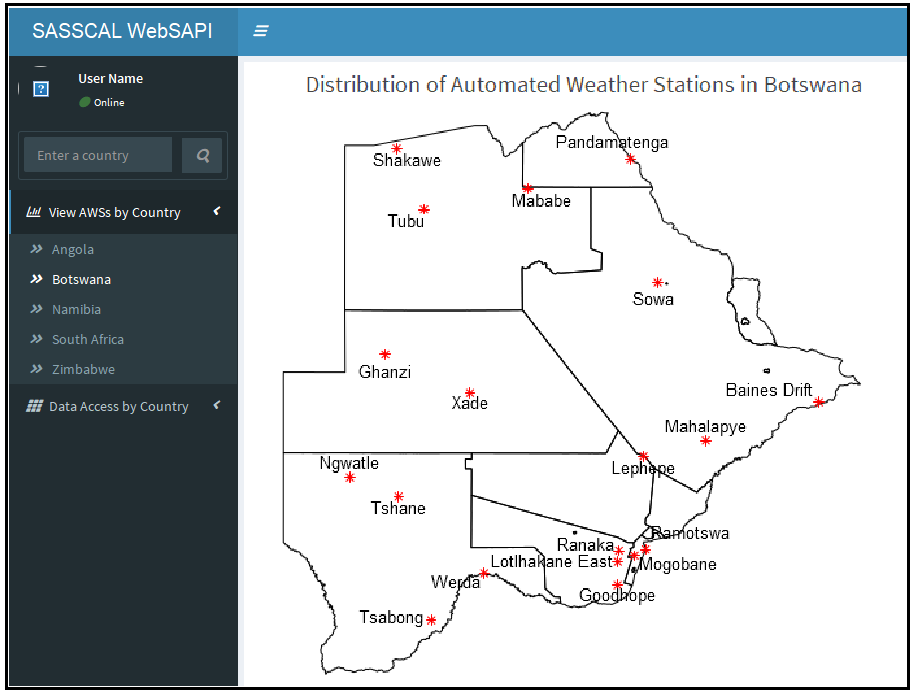
\includegraphics[width=0.9\linewidth]{fig/BW}
	\caption{Screenshot of the SASSCAL WebSAPI for visualisation of SASSCAL's AWSs in Botswana. Maps were generated using the raster package \cite{hijmans2015package} and the maptools package \cite{bivand2013maptools}.  The GUI allows end users to select the geographical location of interest (i.e., Botswana) on the left panel, and a map is visualised on the main panel. 
This is particularly useful for a quick exploration of the geographic locations. % of interest.
	\label{BW}
}
	\label{SASSCAL_WebSAPI}
\end{figure}

\begin{figure}
	\centering
	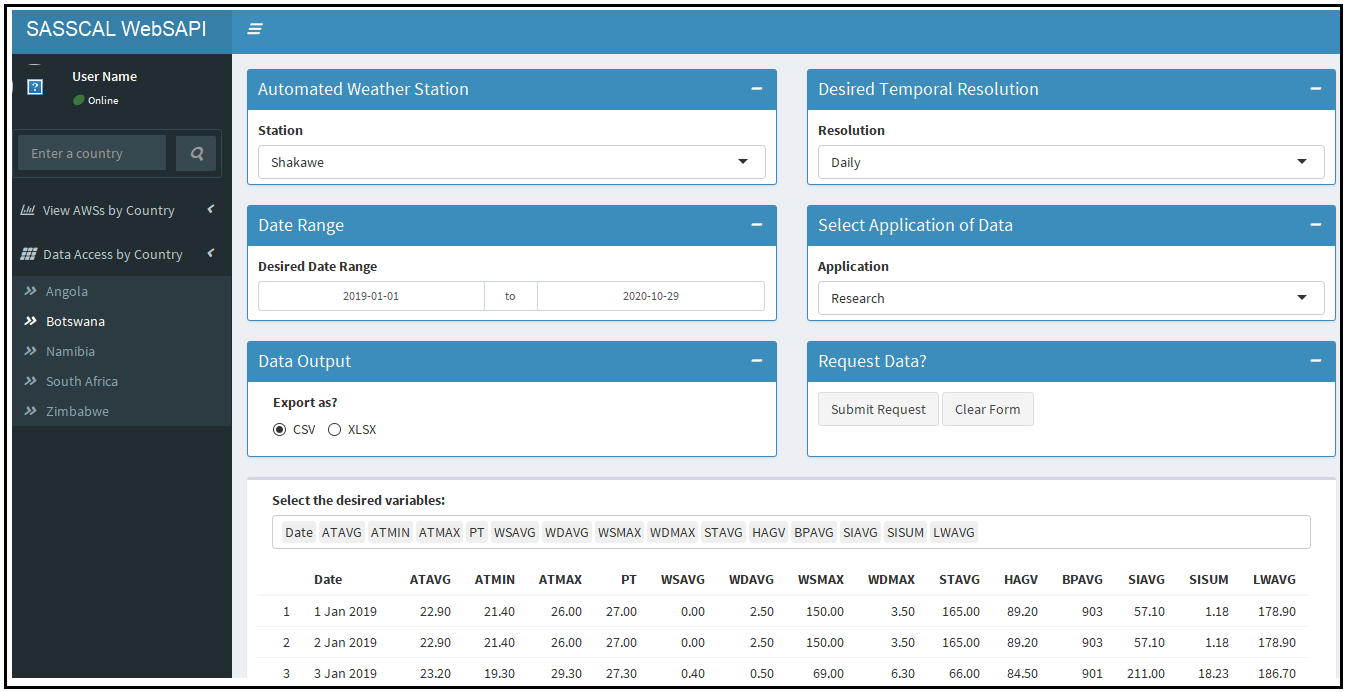
\includegraphics[width=1\linewidth, height=0.4\textheight]{fig/BW_Data}
	\caption{Screenshot of the SASSCAL WebSAPI user interface for data request, visualisation and extraction. 
 The GUI allows end users to select: the desired AWS (i.e., Shakawe AWS),    temporal resolution (i.e., daily),  date range,  use of data, and  the final output's  data format. 
}
	\label{SASSCAL_WebSAPIA}
\end{figure}


\twocolumn
\noindent



%\subsection{Results}
%
\noindent
The  SASSCAL WebSAPI illustrated in Fig. \ref{BW} and Fig. \ref{SASSCAL_WebSAPIA} is a dashboard  based application,  developed to enhance access to the SASSCAL weather data for further use in the world of work.
The WebSAPI also helps in visualisation purposes (using maps, i.e., Fig. \ref{BW} and  tables, see Fig. \ref{SASSCAL_WebSAPIA}). 
The use of the SASSCAL data is motivated by  analysing the distribution of the  average  temperature data using    violin/Box-plots  (see Fig. \ref{BoxP2020}). 
The goal  was to investigate the variations (i.e., peaks) in the  data;  determining whether the temperature values were clustered around the median, the minimum or the maximum. 

\begin{figure}[h]
	\centering
	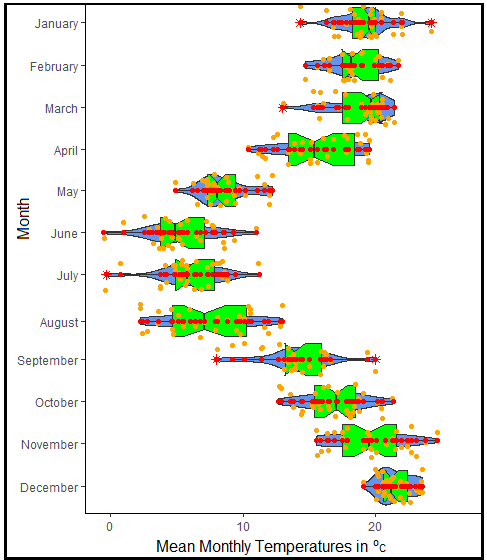
\includegraphics[width=1\linewidth]{fig/BoxP}
	\caption{Violin/Box-plots showing  daily average air temperature distributions   for  Shakawe's AWS (January - December, 2015).
	%	Data will be pulled for the selected SASSCAL AWS ID for the start and end year for each data source for a given time step.
}
	\label{BoxP2020}
\end{figure}

\noindent
As it can be seen in Fig. \ref{BoxP2020}, daily mean temperatures (ATAVG) start increasing from September (commencement of summer), culminating around October-to-January when the sun is overhead at the tropic of Capricorn \cite{WeatherSilitshena}, then they decline gradually through March.  
The ATAVG diminishes gradually from around April until reaching the lowest temperatures (in June and July) leading to a colder season (May to August) which concurs with reports in \cite{moses2017heat,Nkemelang2018}. 
The mean temperature distributions at Shakawe AWS (for 2015) varies with respect to the months.
The shapes of the distribution of June, July and September are extremely skinny on each end and wide in the middle. These indicate the values of the daily mean temperature observations for these months are highly concentrated around the median.
\\
\\
The asterisks ({\color{red}*}) in Fig. \ref{BoxP2020} identify outlier temperatures (in January, March, July, and September), depicting observations outside the 99\% range of a normal distribution represented by the whiskers. The interesting thing about the presentation of data distributions using violin/Box-plots is that outlier temperature values can translate to heat wave observations which are of interest in health, meteorology and agriculture (i.e., high temperatures lead to high evapo-transpiration \cite{moses2018effects}).


\newpage
\section{Discussions}
%  1.Tells the main conclusion of the paper in one or two sentences.
%  2. Tells how the paper’s results contribute to answering the big questions posed in the Introduction.
%  3. Explains how (and why) this work agrees or disagrees with other, similar work.
%  4. Explains how the limitations of this study leave the big questions unanswered.
%  5. Tells how extensions of this paper’s results will be useful for answering the big questions.

\label{Discus}
\noindent
It is well known that no data driven project can start without data \cite{Abbott}. Fortunately, SASSCAL is committed to promote the public dissemination of open science climatic data for research purposes. However, the value of these climatic  data is only useful when it is open and accessible to end users. 
This work contributes with the SASSCAL WebSAPI to enhance access to the  online SASSCAL weather data.
Thus, the SASSCAL WebSAPI extends functionalities of the SASSCAL weathernet to meet end user' requests. It allows reliable and efficacious collection and processing of structured weather data for a preferred temporal resolution based on SASSCAL'  AWSs.  The toolkit extracts the weather data of interest from the SASSCAL weathernet, then unifies  extracted data sets into a downloadable file for further use.\\
\\
%scraping techniques in this weather data, the scraping website presents data publicly. 
%Also, this research does access on a regular basis, does not burden the site (only one request per hour) and does not damage the website hosts of the accessed data.\\
%\\
%We  built the our web scraper using a familiar programming language with availble libraries or packages.  We made this WebSAPI to be   freely accessible by the public just like the SASSCAL Weathernet which is open for scientific research.  %\\
%\\
%The results of data collected are not used for commercial purposes but research purposes. \\
%\\
%The main motivation from extending  the SASSCAL Weathernet has been:    accessing and making use of   the near to real time  weather values generated by through the SASSCAL initiative. % (i.e., for further use in the world of work. 
 %,  violin/Box-plots can aid in %The percentile sizes of the quartiles highlight skewness for the ATAVG distributions (January, March, June, July, September, November and December).
%\subsection{Implications}
%\\%noindent
As a proof of concept, we collected weather data  from the Shakawe  AWS and  analysed the patterns of maximum air temperatures using  violin/Box-plots.
The use of  violin/Box-plots  to analyse environmental data can lead to better understanding of extreme weather events  as also demonstrated  in \cite{Nkemelang2018}. The  work in \cite{Nkemelang2018}
used Box and whisker plots to show the changes in extreme temperature indices   over Botswana based on climate ensemble models.\\
\\
The presentation of the weather outputs  in the form of  violin/Box-plots makes it easier for end users to compare the distributions  of weather data (in this case, average air temperatures) for a given location. This way, end users can have a visual picture of the patterns of weather variables of interest. 
The SASSCAL WebSAPI is  efficient and inexpensive to use, yet with high potential to enhance efficiency in research.
It avoids the time-consuming and repetitive human-engineered and error-prone manual steps of generating data sets.  
This  will be  useful for any researcher; and other practitioners seeking to utilise the SASSCAL weather data in their data driven   projects.
It should be noted as well that this work also contributes by  raising awareness of online SASSCAL scientific data which is open to public. 


\subsection{Limitations}
\noindent
%The SASSCAL WebSAPI requires the integration of several R packages that require the R programming language. However, end users do not need the programming skills to use this app. 
 The   data used for demonstrations  was limited to one year, and collected from one AWS. Hence, the analysis cannot generalise for a larger spatial geographical region. 
 The SASSCAL WebSAPI currently allows the extraction of data from one station at time; using some  user inputs like station name as seen in   Fig. \ref{SASSCAL_WebSAPIA}. 
 There is no capability to extract and analyse data from multiple AWSs at a go.
 This particular functionality can be enhanced by implementing clickable locations on a map of the SASSCAL member country to display the geographic region of interest.
A latitude range functionality could be added to enable efficacious extraction of data from all stations north or south of a certain latitude. 
\\
\\
This toolkit is built on top of the SASSCAL Weathernet. Thus, changes in the structural representation of the SASSCAL weathernet  implies modifications  of this toolkit.  
The  data driven pipeline proposed herein encourages interdisciplinary collaborations to generate appealing  products for end users.
  Lastly, this work opens new pathways for use of these weather data in applied projects. %disruptive applications like smart houses, and energy managements systems. % such as in   government and non-governmental organizations. % as discussed in the following sections.
  %When doing work for government officials who would be interested in the whole district/province, you could include the district shapelife and add a functionality to extract data from all the stations within the district.

\noindent
\newpage
	\section{Conclusion}
	\label{Conclu}
	\noindent
	% short summary of the findings and its meaning for the broad research area.
The SASSCAL WebSAPI aims to   create new channels  to  extend  services of the SASSCAL weathernet.  The toolkit facilitates end users to efficaciously access  and extract  weather data from the  SASSCAL weathernet. 	  
	 	Web scraping and data wrangling techniques  were used to automatically generate weather data sets. A Shiny dashboard was developed to visualise and disseminate outputs to end users. 	 	The toolkit  increases productivity, efficiency and quality of  projects that make use of  data from SASSCAL's AWSs. 
	 	This  toolkit is  valuable  for researchers and analysts who seek to integrate the SASSCAL weather data in their   projects. 
	 	We deployed the toolkit  in a case study to present new statistical analyses of  extreme temperatures in the Okavango Delta.  
	 This toolkit is expected to catalyse many other research  projects like  in the analysis of heat waves \, soil erosivity and erosivity density). 
	 

\section{Recommendations}
\label{Reco}
\noindent
This work motivates the use of  open source technologies to access or visualise data from online climatic data banks.  
The SASSCAL WebSAPI can be scaled to  bridge gaps  of climate data access at local to regional   level. It should be noted that neither the Botswana Department of Meteorological Services nor the Botswana International University of Science and Technology have an API for dissemination of weather and climate information.    Therefore, the SASSCAL WebSAPI  can be adapted and incorporated to portals of weather service providers (like BIUST and SASSCAL) to facilitate open access to weather data.
All these could enable end users to  quickly explore 	several weather data sets and  summarise their statistics to make well informed decisions regarding their data source and sample sizes for use in their 	research projects.

	
\section{Future Directions}
\label{Futuro}
\noindent
This work  will continue to motivate and encourage the use of weather and climate data that is normally archived and left under utilised, especially in developing regions like Africa. 
More end user-driven functionalities will be added to this API to: (1) improve the user interface to enhance access mechanisms to the SASSCAL weathernet; (2)  monitor the research data be accessed; and (3)  investigate strategies for imputation of missing weather data using the historical  SASSCAL weather data. The analysis and visualisation of SASSCAL weather data for multiple AWSs will be conducted to capture the spatial-temporal resolutions of various weather parameters   to enhance the understanding of relationships between the collected weather variables at local levels.
 
	%%%%%%%%%%%%%%%%%%%%%%%%%%%%%%%%%%%%%%%%%%%%%%%%%%%%%%%%%%%%%%%%%%%%%%%%%%%%%%%%
	\section*{Acknowledgements}
	\noindent
We thank the Botswana International University of Science and Technology for the partial financial support (with reference number: S-00086).	We thank  % Botswana International University of Science and Technology for supporting this work; and 
 the Southern   African   Science   Service   Centre for  Climate  and  Land  Management    for availing the weather data used in this work.


\section*{Conflict of interest}
None

\section*{Reproducibility}
This  work is an open source   R based toolkit under development.  The code is available on \url{https://github.com/EL-Grande/SASSACL-WebSAPI}. %github: https://github.com/cocomice/EDSS_dep_framework
\newpage

\bibliographystyle{ieeetr}
\bibliography{MiBib}
\clearpage
\end{document}
